\begin{flushright}
    در قسمت قبل با ساختار HDDها آشنا شدیم.
    در این قسمت می‌خواهیم به طور انتزاعی و از نگاه نرم‌افزاری بار دیگر به بررسی این حافظه‌ها بپردازیم.

    \begin{figure}[H]
        \centering
        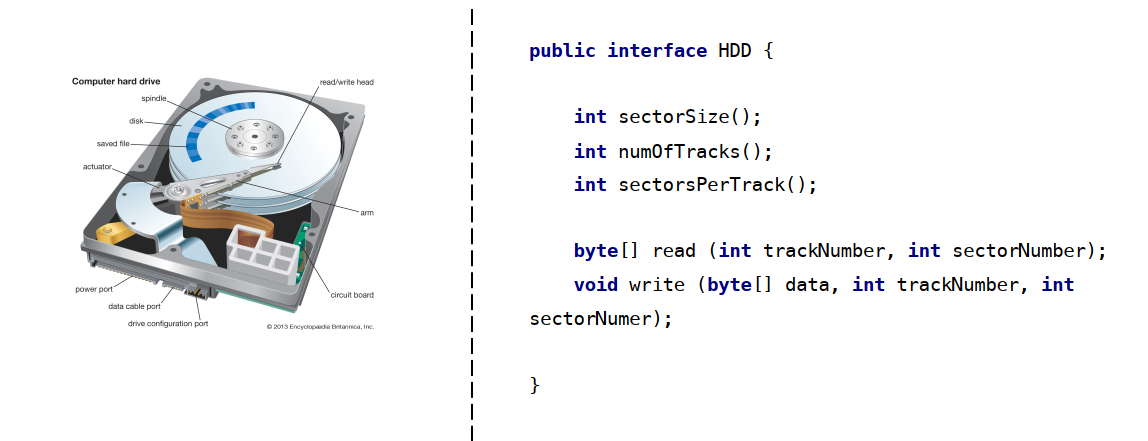
\includegraphics[width=\textwidth]{source/hdd-abstract-view}
        \caption{نگاه انتزاعی به HDD}
        \label{fig:hdd-abstract-view}
    \end{figure}

    در این نگاه، حافظه شامل تعدادی بلوک حافظه و تعدادی شیار است و همچنین دو تابع برای خواندن و نوشتن بر روی این بلوک‌ها دارد.

    فرض کنید می‌خواهیم یک حافظه برای ذخیره‌سازی داده‌های دانش‌آموزان ایجاد کنیم.
    اطلاعات دانش‌آموزان به صورت زیر است:

    \begin{figure}[H]
        \centering
        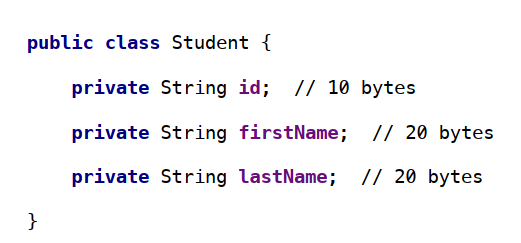
\includegraphics[width=0.6\textwidth]{source/student-data-model-1}
        \caption{اطلاعات دانش‌آموزان}
        \label{fig:student-data-model-1}
    \end{figure}

    با فرض آنگه اطلاعات هر دانش‌آموز در یک بلوک حافظه ذخیره می‌شود، می‌توانیم این اطلاعات را به صورت زیر در حافظه ذخیره کنیم:

    \begin{figure}[H]
        \centering
        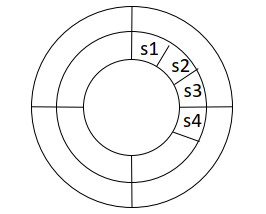
\includegraphics[scale=1]{source/student-on-HDD}
        \caption{نجوه ذخیره‌سازی اطلاعات دانش‌آموزان در حافظه}
        \label{fig:student-on-HDD}
    \end{figure}

    از نگاه نرم‌افزاری، نیز با داده ساختاری به شکل زیر روبرو هستیم.

    \begin{figure}[H]
        \centering
        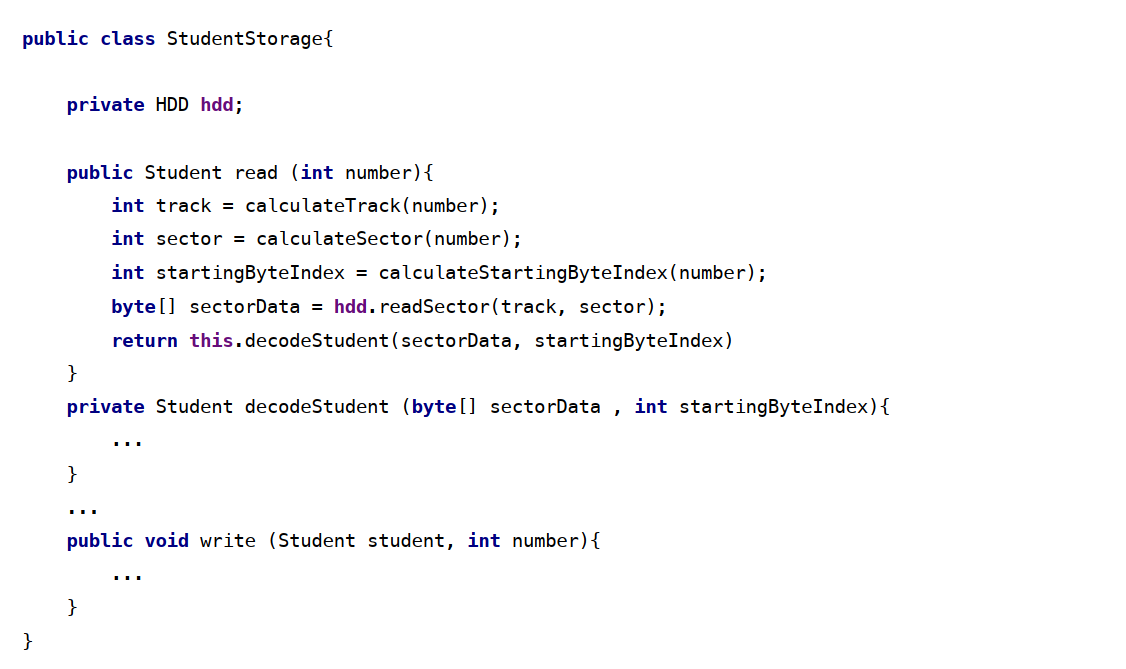
\includegraphics[scale=0.41]{source/student-storage-model-1}
        \caption{نگاه نرم‌افزاری به حافظه ذخیره‌سازی اطلاعات دانش‌آموزان}
        \label{fig:student-storage-model-1}
    \end{figure}

    حال فرض کنید می‌خواهیم از نوع دیگری از حافظه استفاده نماییم.
    مشخص است که تغییراتی در پیاده‌سازی \emph{storage student} مورد نیاز است.

    \begin{figure}[H]
        \centering
        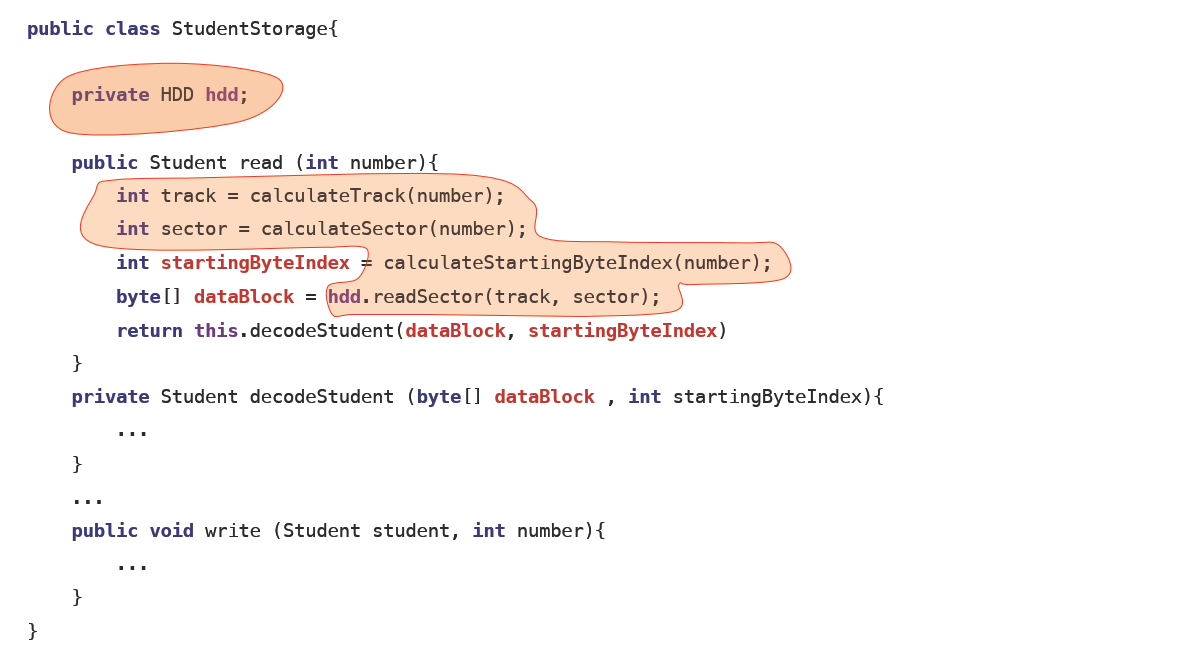
\includegraphics[scale=0.41]{source/student-storage-model-1-hardcoded}
        \caption{قسمت‌هایی که در پیاده‌سازی نیاز به تغییر دارند}
        \label{fig:student-storage-model-1-hardcoded}
    \end{figure}


    پیاده‌سازی را طوری تغییر دهیم تا از نوع حافظه مورد استفاده مستقل باشد، نیاز به یک انتزاع بر روی حافظه می‌باشیم.
    برای این مهم، می‌توانیم حافظه را به چشم یک سری بلوک پشت سر هم در نظر بگیریم.
    در اثر این شکل از انتزاع کافی است تا واحد‌های ذخیره‌سازی حافظه‌های مختلف را به این بلوک‌ها مپ کنیم.

    \begin{figure}[H]
        \centering
        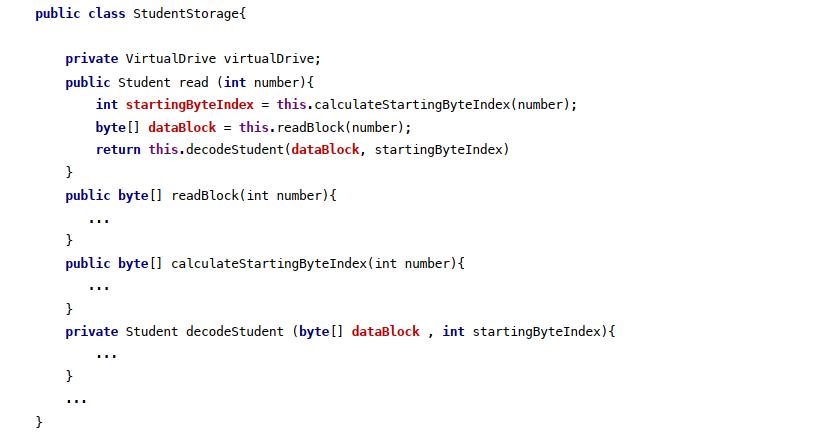
\includegraphics[scale=0.6]{source/student-storage-model-2}
        \caption{مستقل کردن پیاده‌سازی از نوع حافظه}
        \label{fig:student-storage-model-2}
    \end{figure}

    \begin{figure}[H]
        \minipage{0.5\textwidth}
        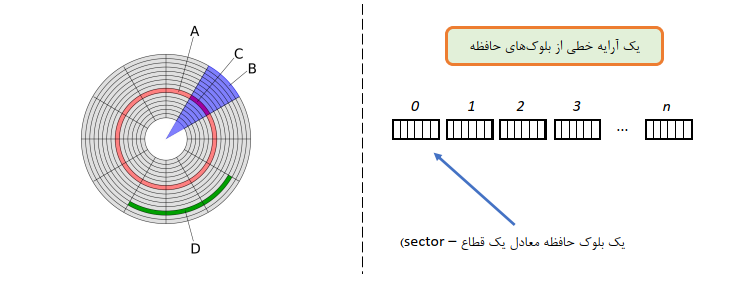
\includegraphics[width=\linewidth]{source/HDD-to-Drive}
        \label{fig:HDD-to-Drive}
        \endminipage\hfill
        \minipage{0.5\textwidth}
        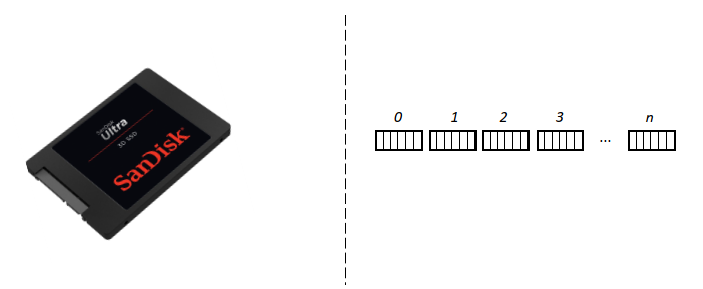
\includegraphics[width=\linewidth]{source/SSD-to-Drive}
        \label{fig:SSD-to-Drive}
        \endminipage\hfill
        \minipage{0.5\textwidth}
        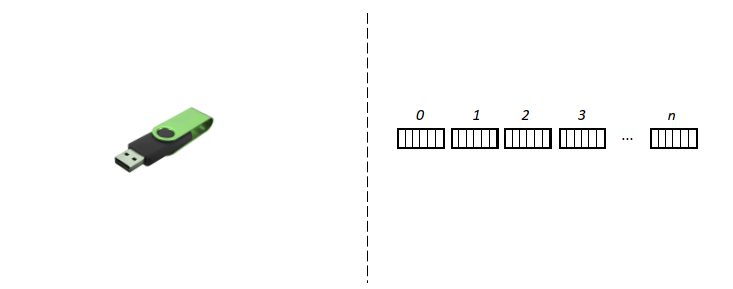
\includegraphics[width=\linewidth]{source/flash-to-Drive}
        \label{fig:flash-to-Drive}
        \endminipage\hfill
        \minipage{0.5\textwidth}
        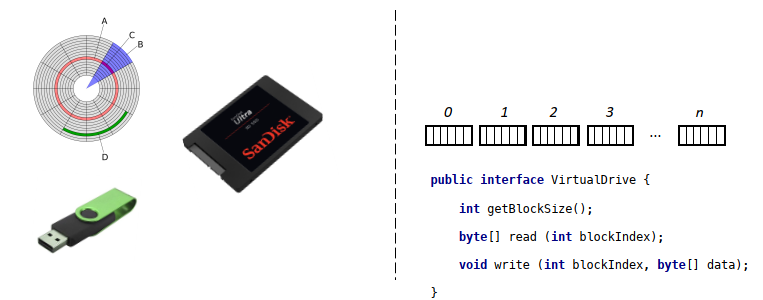
\includegraphics[width=\linewidth]{source/all-to-Drive}
        \label{fig:all-to-Drive}
        \endminipage\hfill
    \end{figure}

    \newpage
    این نحوه از پیاده‌سازی دو تاثیر مهم دارد.
    \begin{enumerate}
        \item برنامه را مستقل از تکنولوژی مورد استفاده می‌کند. ( Principle Inversion Dependency   )
        \item اگر در آینده تصمیم بر اضافه کردن یک فیچر کردیم، تغییری در پیاده‌سازی ما ایجاد نشود. ( Principle Open-Closed )
    \end{enumerate}

    \begin{figure}[H]
        \minipage{0.5\textwidth}
        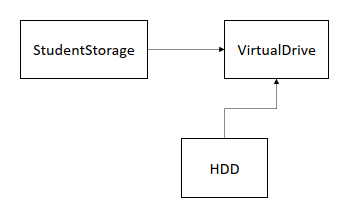
\includegraphics[width=\linewidth]{source/DIP}
        \caption{Principle Inversion Dependency}\label{fig:DIP}
        \endminipage\hfill
        \minipage{0.5\textwidth}
        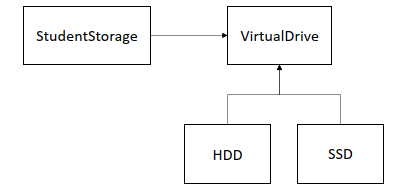
\includegraphics[width=\linewidth]{source/OCP}
        \caption{Principle Open-Closed}\label{fig:OCP}
        \endminipage\hfill
    \end{figure}

\end{flushright}